% * How many of original goals were achieved? Proved to have been achieved
% * Did the program really work?
% *! Credit for interesting conclusion

% ************
% Should have: 
% 	intro
% 	content
% 	summary
% ************

% What I want to say
%
% Questions to answer:
% * Are Distributed Hash Tables viable data stores for a distributed search engine?
% * Do they scale with size?
% * How do Chord and Pastry compare?
%
% Discuss how started with factorial design with factors of nodes and rate.
% Found doesn't vary over length of run, so any run viable.
% All data from three separate runs.
%
% What looked at was latency and success rate.
% 
% Findings to comment on:
% * Why is Chord so much slower than Pastry?
% * Why does Chord has such a low yield rate compared to Pastry
%
% Conclude
% * Does it work for search engine?

\section{Evaluation}
% TODO: Summarize what I am about to say

\subsection{What to test}
% Questions to answer:
% * Are Distributed Hash Tables viable data stores for a distributed search engine?
% * Do they scale with size?
% * How do Chord and Pastry compare?
% What looked at was latency and success rate.
The approach I will take when evaluation the Distributed Hash Tables Chord and Pastry is quantitative. Their correctness and underlying theory has been widely discussed in research papers and I have nothing new to contribute there. What interests me is if they could work well as data stores in the distributed friend search engine I am proposing to build. To that extent what I will be evaluating is the latency of key lookups, and the success rate of lookups in the network.

We will also look at how they scale with size, and pit Chord against Pastry to see which one performs best.

\subsection{Experimental design}
% Discuss how started with factorial design with factors of nodes and rate.
% Found doesn't vary over length of run, so any run viable.
% All data from three separate runs.
I ran my system on top of machines in the Planet-Lab network. With that in mind, the variables I was able to control where the number of machines participating in the system, the number of Distributed Hash Table nodes running on each machine, and the rate of requests in the network.

In my tests I used all the machines available to me to give some scale to the experiments, and limited the experimental factors to the number of nodes run on each machine and the rate at which requests were issued.

I decided on a factorial design where both node count and rate varied between 1 and 16 in powers of two. For both Chord and Pastry each configuration was run at three different occasions. The three log files combined were then used to give the results I am about to present.

\subsubsection{Experimental pattern}
Each experimental run followed a predefined pattern:
\begin{enumerate}
\item I would ensure that correct number of nodes was running
\item If the number of nodes had to be adjusted, the nodes would be given 3 minutes to update their routing tables.
\item Each machine would clear its previous logs and start its logging machinery.
\item After that the actual experiment would start. Each machine would issue requests to the nodes it hosted at a rate specified for that particular experimental run.
\item After a successfully completed run, there would be a cool down period with continued logging where requests taking slightly longer than permitted would be allowed to finish. Logging would then stop and the logs from the individual machines would be collected at the central hub node.
\item The logs where then downloaded from the central hub to my personal machine for safe keeping and analysis.
\item The process was then repeated for a different set of parameters.
\end{enumerate}

\subsection{Effects of Planet-Lab}
As previously mentioned my experiments ran on top of machines provided by Planet-Lab. I was allowed to run up to 100 machines, but did never manage to get quite that many up and running at the same time.

Using Planet-Lab as a test bed gave me several benefits: the machines at my disposal had a high geographical spread, and varied greatly in what computational resources they provided. Depending on the time of day the computational load on the machines would also vary and not only that, but I would have a different subset of the machines available for testing from day to day.

This infrastructure provided an excellent foundation to test Distributed Hash Tables which are meant to be able to cope with high node churn and machines with widely different capabilities.

While Planet-Lab provides an interesting test bed, its natural variability also makes experiments impossible to accurately repeat. Repeating the same experiment at a different time would invariably give a slightly different result.
To work with Planet-Lab's strengths and not against it, and to at the same time get data I could have confidence in, I ran each experiment repeatedly, shifted in time. This way I ensured I would sample different subsets of the topology. I believe this gives me results that while having higher variance, also more closely resemble the real world scenario Distributed Hash Tables are likely to find themselves in.

\subsubsection{Experimental cleanliness and validity of results}
Performing experiments over longer periods of time showed that the success rate (figure \ref{figLatencyAgainstTime}) and latency (figure \ref{figRateAgainstTime}) stayed constant over time. This allowed me to cut down the length of individual experiments without lowering the quality of my results.

\begin{figure}[!htb]
  \begin{center}
    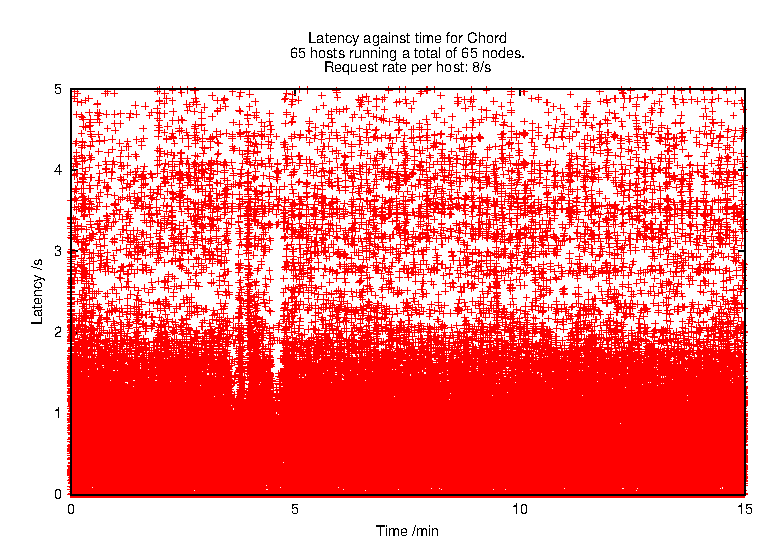
\includegraphics[]{illustrations/latency_aginst_time_chord.eps}
    \caption{This graph shows how latency varies over time in a 15 minute experimental run of Chord.}
    \label{figLatencyAgainstTime}
  \end{center}
\end{figure}

\begin{figure}[!htb]
  \begin{center}
    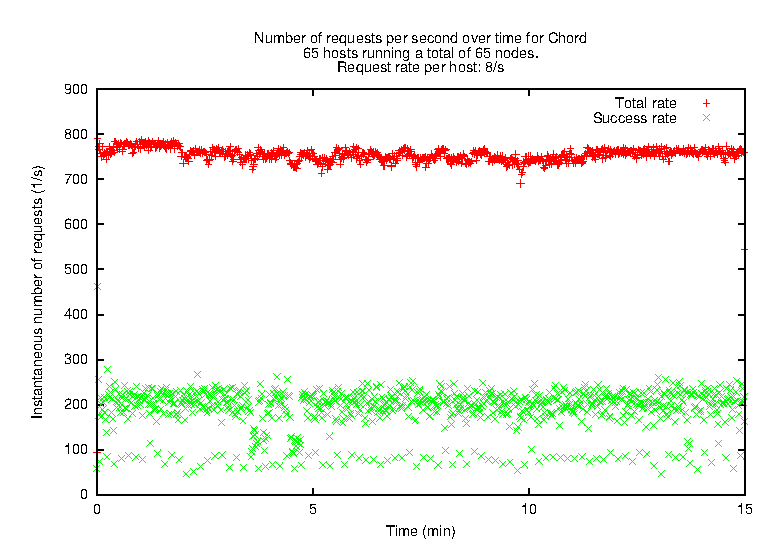
\includegraphics[]{illustrations/rate_against_time_chord.eps}
    \caption{This graph shows how the request rate and success rate varies over a 15 minute experimental run of Chord.}
    \label{figRateAgainstTime}
  \end{center}
\end{figure}

% * How logging not affect results
During experimental runs I would turn of all functionality not directly needed for serving the requests. This would include turning of the mechanisms that kept the nodes routing tables up to date. This initially sounds slightly problematic. If a Distributed Hash Table node disappeared during an experiment, nodes contacting it directly would take note of it, but other nodes wouldn't have the nodes disappearance reflected in their routing state like they would under normal operation. This might seem a somewhat unnatural choice, but makes sense for my experiments for the following reasons:

In my experimental builds of Chord and Pastry I had turned up the rate a which routing information was dissipated through the network to an extreme to make experimental runs shorter. Since what I wanted to test was the raw performance of the system, removing the overhead from keeping the routing tables up to date made sense, especially since this overhead differed between Chord and Pastry, and is a parameter that would have to be tweaked before using this system in any real world deployment.
Also having established that the length of the experimental runs was insignificant made me confident in that not updating routing information during experimental runs did no harm to the experimental results.

% * How load spread evenly
\mbox{}
To ensure even load across my test network, each machine involved individually issued requests to the Distributed Hash Table network.
Keys to access were randomly generated by hashing a combination of the node Id and a time stamp. The result of using this approach is that the keys used for testing differ from experimental run to experimental run. While this makes doing repeatable experiments impossible, it nicely models a real world spread of keys that otherwise would be hard to predict and also evenly spreads the loads between the machines.

% * What constitutes a valid run
Runs where machines vanished during runs would be discarded.


\subsection{Results and comments on results}
Throughout my experiments, a valid request is defined as a request that completes within 5 seconds. By that definition, all other requests are invalid, regardless of if they fail to complete at all, or if they just complete after more than 5 seconds have passed.
% Comment on what is a valid request. And what is considered a failed request
% Findings to comment on:

\subsubsection{Mean latency and success rate for Chord and Pastry}
In figure \ref{figChordLatency} and \ref{figPastryLatency} you see the latency for different rates and different number of nodes per machine for around 60 machines, shown with 95\% confidence intervals. 

What is immediately striking is how much more variance there is in the latencies for Chord than there is in the latencies for Pastry.
In the case of Pastry (figure \ref{figPastryLatency}) we see how the latencies consistently grow for larger number of nodes. Intuitively this is what we would expect as the theory behind the Distributed Hash Tables tells us the number of nodes involved in a look up is proportional to the logarithm of the number of nodes in the network. The same trend is not apparent for Chord (figure \ref{figChordLatency}). On the contrary there is no apparent correlation between the number of notes and the latency for a given rate. What is also peculiar is that, looking at the latencies for a fixed number of nodes per host, the latencies seem to decrease under higher load!

\begin{figure}[htb]
  \centering
  \subfigure[Latency for Chord]{
    \label{figChordLatency}
    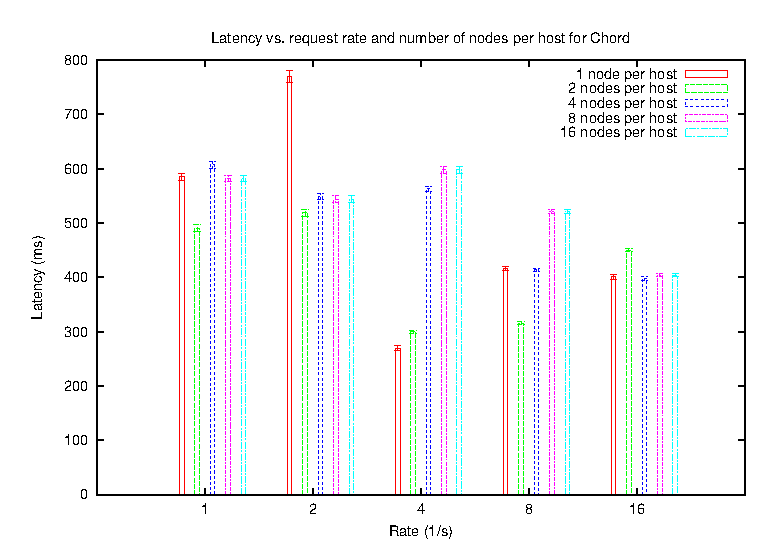
\includegraphics[]{illustrations/latency_chord.eps}
  }
  \subfigure[Success rate for Chord]{
    \label{figChordSuccessRate}
    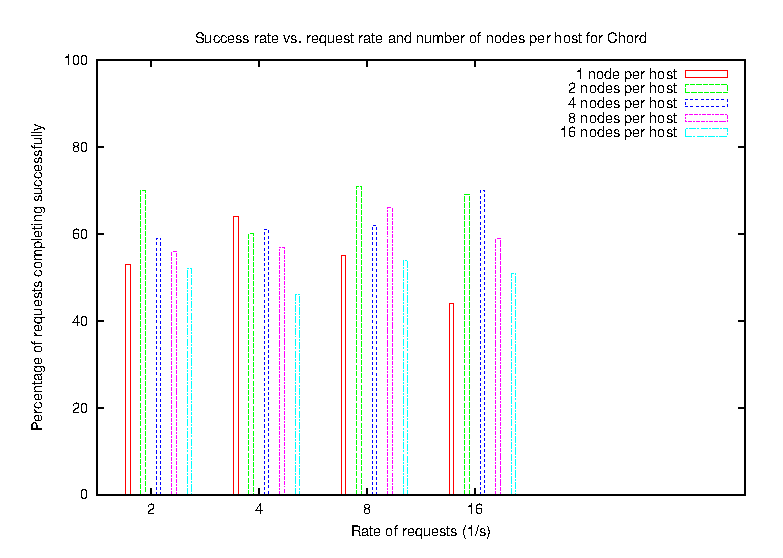
\includegraphics[]{illustrations/success_rate_chord.eps}
  }
  \caption{The graphs above show (a) latencies with 95\% confidence intervals, and (b) success rate for a Chord setup of slightly above 60 nodes.}
\end{figure}

\begin{figure}[htb]
  \centering
  \subfigure[Latency for Pastry]{
    \label{figPastryLatency}
    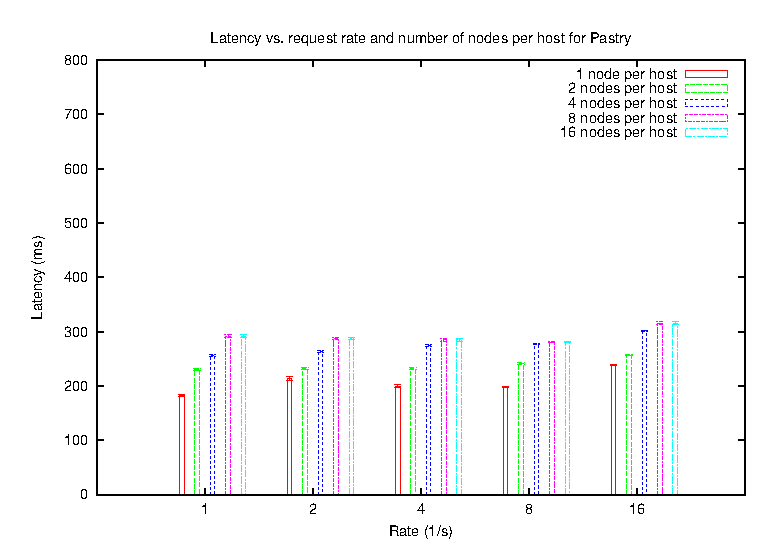
\includegraphics[]{illustrations/latency_pastry.eps}
  }
  \subfigure[Success rate for Pastry]{
    \label{figPastrySuccessRate}
    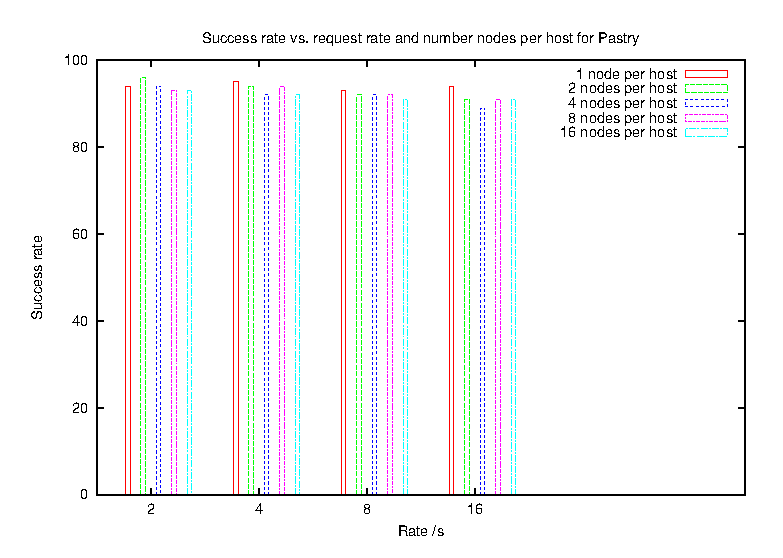
\includegraphics[]{illustrations/success_rate_pastry.eps}
  }
  \caption{The graphs above show (a) latencies with 95\% confidence intervals, and (b) success rate for a Pastry setup of slightly above 60 nodes.}
\end{figure}

The success rate Chord (figure \ref{figChordSuccessRate}) and Pastry (\ref{figPastrySuccessRate}) is also dramatically different. Chord seems to perform better when more than one node is run on the same machine, while Pastry's success rate slightly decreases the more nodes are run on the same physical hardware. It is also worth noting that at its best, Chord can't compare with the performance of Pastry.

Unfortunately I have no good explanation for the variations we see within the different configurations for Chord, but I can explain why Chord in the general case performs so much worse than Pastry does and I will do so shortly.

Before that I want to discuss how Chord and Pastry behave when pushed to their limits. The cumulative distribution functions for Chord (figure \ref{figChordCDF}) and Pastry (figure \ref{figPastryCDF}) show the percentage of requests that succeed within five seconds. Each in both cases the experiments are run on roughly 60 machines hosting 1 node each. We see how the success rate in the case of Pastry slowly drops as we get to 128 requests per second per machine.

In the case of Chord on the other hand, the success rate is only marginally worse for 128 and 64 requests per second per hosts than they are when there are 16 requests per second per machine. Also rather odd in the case of Chord is how the rate of 2 per second performs significantly worse than what does the rate of 4. I have no good explanations for this behaviour.

\begin{figure}[htb]
  \centering
  \subfigure[Cumulative distribution function of success against latency for Chord]{
    \label{figChordCDF}
    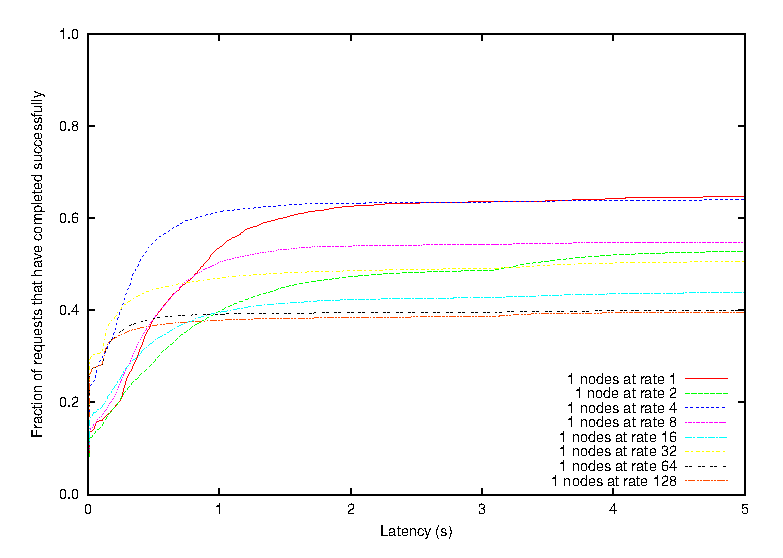
\includegraphics[]{illustrations/cdf_chord.eps}
  }
  \subfigure[Cumulative distribution function of success against latency for Pastry]{
    \label{figPastryCDF}
    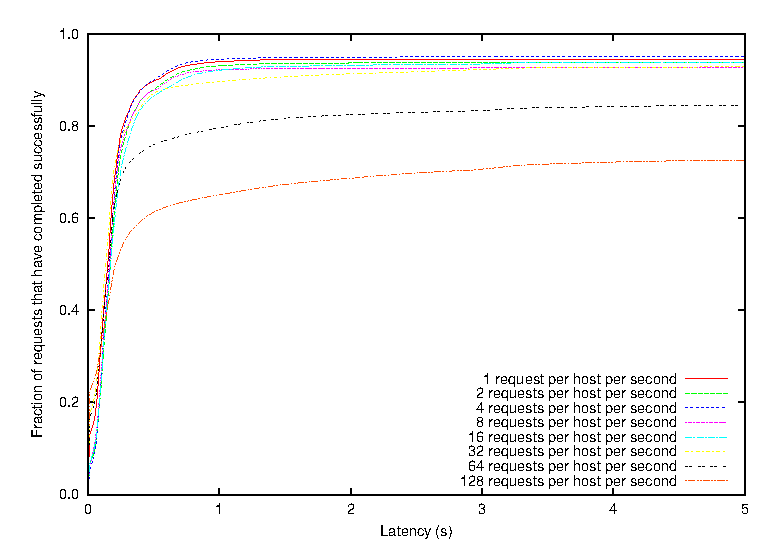
\includegraphics[]{illustrations/cdf_pastry.eps}
  }
  \caption{The graphs above show the cumulative distribution function of a request being successful within the first 5 seconds for (a) Chord, and (b) Pastry.}
\end{figure}

\subsubsection{Why does Chord perform worse that Pastry}
The experimental evidence shown so far clearly shows Pastry as superior to Chord both in terms of latency and in the success rate of requests. I will now try to explain in turn what the cause might be.

\mbox{}

The higher latencies of Chord are the easiest to explain. In figure \ref{figChordNumNodes} and \ref{figPastryNumNodes} you see how many nodes are involved in a particular key lookup in Chord and Pastry respectively. It is clear from the graph that the average number of nodes involved in a key lookup are greater for Chord than for Pastry. If one multiplies the average time it takes to setup a TCP connection with the number of nodes involved, it should be clear that a Chord lookup should take longer if the only thing one is accounting for is the latency of the routing. We are also not factoring in that Pastry uses a heuristic favouring nodes closer by in routing, which additionally should affect the latency as each routing step is likely to take less time than it does for Chord. I will shortly discuss the impact of the proximity heuristic in Pastry.
If the higher number of routing steps for Chord is a bug introduced by me or something inherent to the Chord algorithms is something I can't comment on. It is also possible that the difference would become less significant for larger networks of nodes. Unfortunately this is not something I was able to test given the infrastructure available to me.

\begin{figure}[htb]
  \centering
  \subfigure[Number of nodes involved in key lookup for Chord]{
    \label{figChordNumNodes}
    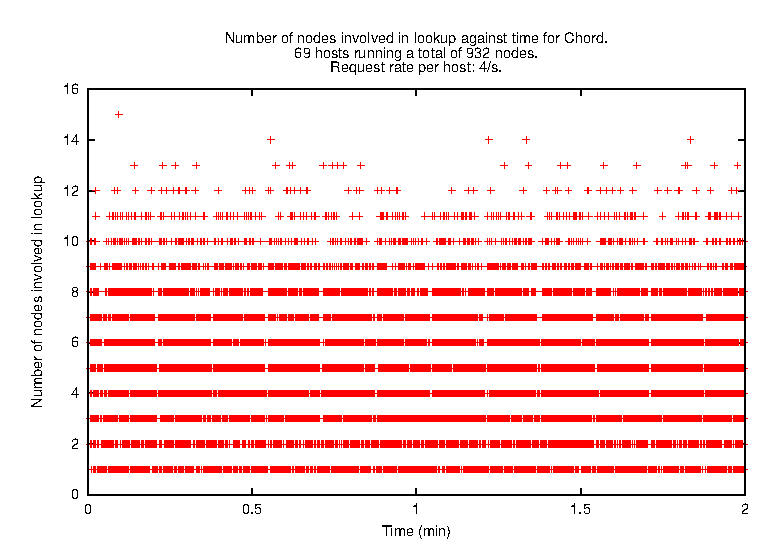
\includegraphics[]{illustrations/nodes_against_time_chord.eps}
  }
  \subfigure[Number of nodes involved in key lookup for Pastry]{
    \label{figPastryNumNodes}
    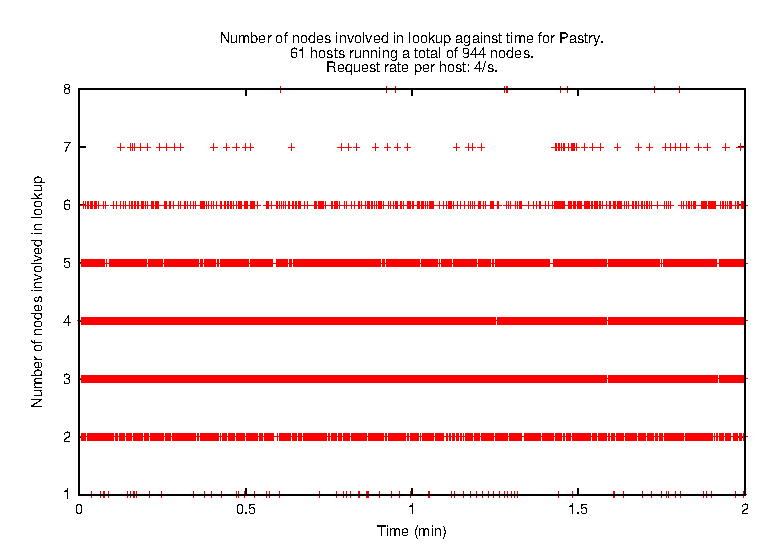
\includegraphics[]{illustrations/nodes_against_time_pastry.eps}
  }
  \caption{The graphs show the number of nodes involved in a key lookup for (a) Chord and (b) Pastry for a particular experimental run.}
\end{figure}

\mbox{}
Now that we have an idea of why the latency might be higher for Chord than for Pastry, let me try to explain why the failure rate might also be higher.

First we let us recall how Chord and Pastry perform their routing.
In Chord, the node that wants to lookup a key (the requester) asks the closest node to the key if they know about other nodes closer to the target key than itself. It then asks the node it gets returned the same question, and the pattern continues until it finds the node preceding the key. Its successor is the target node responsible for the key.

Pastry on the other hand follows a different approach. When a requesting node looks up a key is again makes a request to the node it knows about that is closest to the target node. What differs from the Chord approach though is that the requester hands over the responsibility for the continued lookup to the node it asked. This node in turns then asks another node until the target node has been reached.

Now lets consider what happens when something goes wrong.
In figure \ref{figChordFailedLookup} we see what happens when Chord node A gets returned node D as the next hop node from B. D is not accessible and the lookup fails. If the routing is retried B again returns D, unless it in the meantime itself has noticed that D is inaccessible.

In the Pastry case on the other hand node B becomes responsible for routing the request forward towards the target node. Upon realising node D is unavailable it routes it to the next closest node it knows about, in this case C. Node C happens to know about a closer node to the target than B and this way we managed to route around the dead node D.

There are workarounds to improve the performance of the Chord routing. One would be for the requesting node A to inform node B about node D's death upon retrying to route the message. An alternative could also have been for A to try to route the request through another intermediate node before D, but in this case we are not guaranteed that this intermediate node will not also return D.
A third approach could be to look up D's predecessor, and then use that node in the same role that B filled in this example. None of these methods have been implemented in my implementation as they would extend the core Chord routing algorithm and therefore skew the comparison in Chord's favour.

\begin{figure}[htb]
  \centering
  \subfigure[Failed lookup in Chord]{
    \label{figChordFailedLookup}
    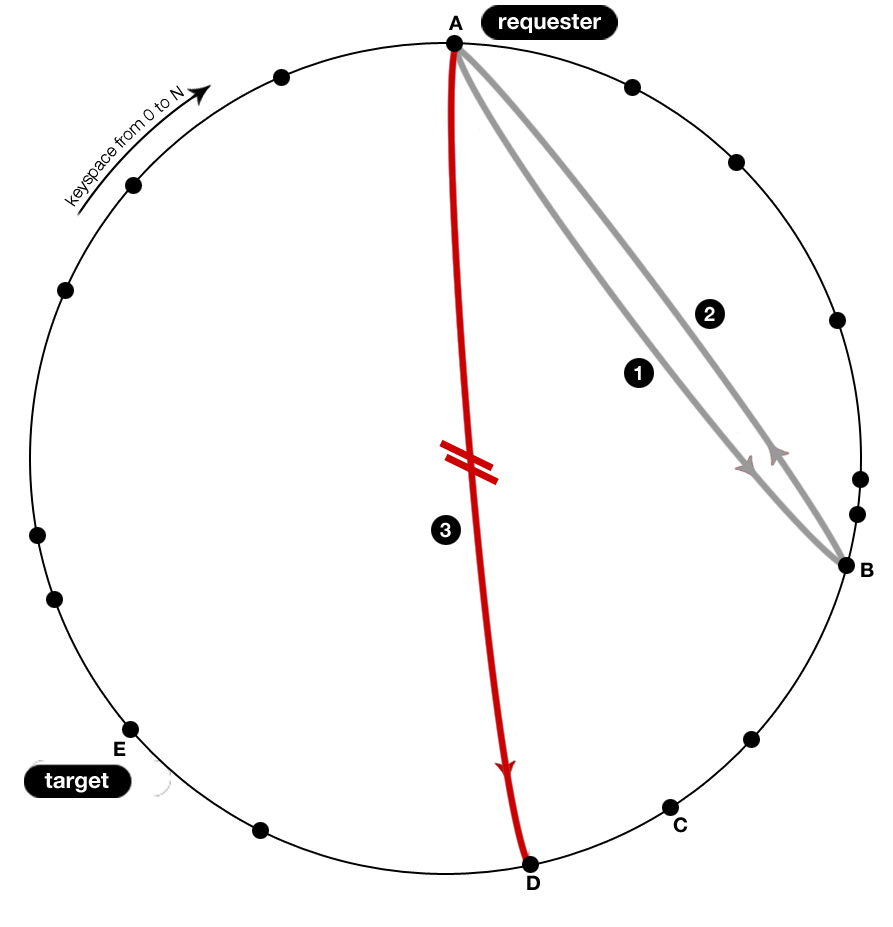
\includegraphics[]{illustrations/ChordRoutingFailed.png}
  }
  \subfigure[Failed lookup in Pastry]{
    \label{figPastryFailedLookip}
    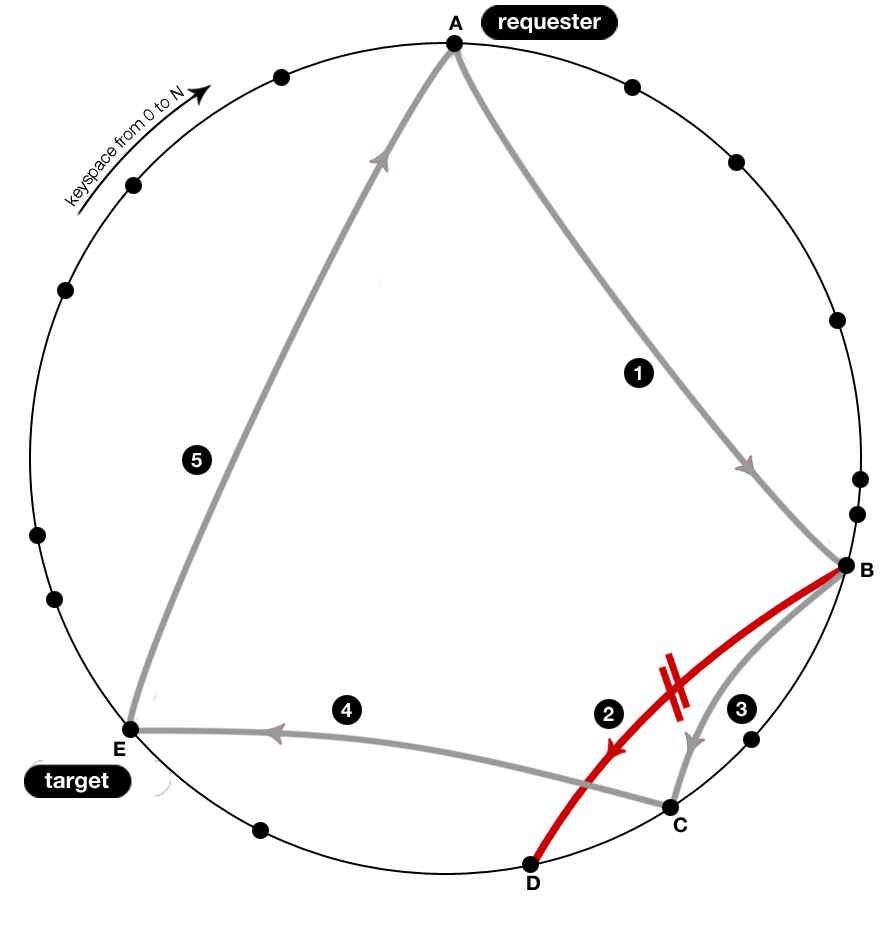
\includegraphics[]{illustrations/PastryRoutingFailed.png}
  }
  \caption{The illustrations show the differences in the routing approach of Chord and Pastry in the case where one of the nodes in the lookup chain is not accessible (Node D). In the case of Pastry it routes around the failed node, while Chord if trying to route again will again get node D returned by node B.}
\end{figure}

% * Why is Chord so much slower than Pastry?
% * Why does Chord has such a low yield rate compared to Pastry
% * How much can we conclude from the numbers?

\subsection{Effect of Pastry routing heuristics}
% * What effect does the Pastry routing heuristics have on the performance
In this section I will try to get a measure to what extent the proximity heuristic used by Pastry affects its routing performance. Be warned that it is rather speculative and relies on some assumptions that cannot necessarily be generalized, but none the less I feel it is interesting food for thought. I will clearly state where I am making assumptions that do not necessarily hold.

The approach I will take is as follows.
This experiment uses a total of 50 nodes. First we look at what overhead is when moving from 50 nodes on 50 different machines to running 5 nodes on each of 10 machines. Since Chord uses no heuristic, we can easily get numbers for how this move affects the routing performance in Chord. In order to relate this Pastry we need a measure for how Pastry and Chord compare when there is no heuristic being used at all. This is rather tricky as the heuristic is tightly integrated into the way Pastry performs its routing. I got this measure by running 50 nodes on a local node on a powerful machine. Since all inter-node communication is on the same machine, the latency is negligible and the routing heuristic plays no part. 

By then comparing the actual impact of moving from 50 machines with one node each to 10 machines with 5 nodes each in the performance of Pastry and comparing the results with what I would have expected them to be, I can estimate how much of an impact the routing heuristic actually had.

The result we get is not necessarily general though, and applying it to random Pastry deployments would be unwise. The results still give an interesting pointer to if such heuristics are beneficial or not.

% TODO: Write shit

I will look at what the overhead is when moving the 100 nodes from 50 separate machines with two nodesfor how much of an impact the Pastry proximity heuristic has on Pastry's routing performance. It is very hard to isolate the effects caused by the heuristic as there are very manywant to quantify to what extent the proximity heuristics used by Pastry increase its performance. 


\subsection{Viability of Distributed Hash Tables a backend store for a search engine}
% Conclude
% * Does it work for search engine?

% TODO: Summary of what we have discussed in this chapter.
